\subsection{Dynamic DMR Prediction and Recalibration}

Because patient-level cumulative DMR probability was underpredicted in the development cohort, we developed an exploratory dynamic prediction and recalibration analysis. At each landmark time \(s\), the target estimand was the probability of documented DMR by \(s+H\) among patients who were DMR-free at \(s\):
\[
\Pr(T_i^{\mathrm{DMR}}\le s+H \mid T_i^{\mathrm{DMR}}>s,\mathcal H_i(s)),
\]
where \(\mathcal H_i(s)\) denotes the MRD history available up to the landmark. Landmarks were set at 6, 12, 18, and 24 months. Prediction horizons were 6, 12, and 24 months. A landmark record was included only if the patient had at least one MRD measurement at or before the landmark and the horizon outcome was observable, defined as documented DMR by \(s+H\) or follow-up beyond \(s+H\).

For posterior draw \(m\), the original dynamic prediction was computed from the fitted joint model as
\[
p_i^{(m)}(s,H)=
1-\exp\{-H h_i^{(m)}(s,H)\},
\]
where
\[
h_i^{(m)}(s,H)=
\exp\{\gamma_0^{(m)}+\gamma_1^{(m)}\log(1+t^{mid})
+\gamma_2^{(m)}\log(1+H)+\alpha^{(m)}\eta_i^{(m)}(t^{mid})\},
\]
and \(t^{mid}=s+H/2\). The posterior mean prediction was
\[
\hat p_i(s,H)=M^{-1}\sum_{m=1}^{M}p_i^{(m)}(s,H).
\]
To address calibration-in-the-large and possible over- or under-dispersion, horizon-specific logistic recalibration was then fitted:
\[
\mathrm{logit}\{p_{i,\mathrm{cal}}(s,H)\}
=
a_H+b_H\mathrm{logit}\{\hat p_i(s,H)\}.
\]
Performance was summarized using the dynamic Brier score, calibration intercept, calibration slope, and grouped observed-versus-predicted calibration plots. Clustered bootstrap resampling by patient was used to estimate optimism in the recalibration layer. The full Bayesian joint model was not refitted in bootstrap samples.

\begin{table}[!htbp]
\centering
\caption{Development-cohort dynamic prediction and recalibration performance. Predictions are landmark-level probabilities of documented DMR by the stated horizon among patients who were DMR-free at the landmark and had at least one prior MRD measurement. Optimism correction applies to the recalibration layer only; the Bayesian joint model itself was not refitted in bootstrap samples.}
\label{tab:dynamic-prediction-validation}
\resizebox{\linewidth}{!}{%
\begin{tabular}{llrrrrrrrr}
\toprule
Horizon & Model & n & Events & Observed & Mean predicted & Brier & Opt.-corrected Brier & Cal. intercept & Cal. slope \\
\midrule
6 months & Original posterior & 108 & 39 & 0.361 & 0.506 & 0.179 & 0.179 & -1.00 & 0.85 \\
6 months & Recalibrated & 108 & 39 & 0.361 & 0.361 & 0.157 & 0.167 & -0.00 & 1.00 \\
12 months & Original posterior & 99 & 57 & 0.576 & 0.626 & 0.162 & 0.162 & -0.36 & 0.81 \\
12 months & Recalibrated & 99 & 57 & 0.576 & 0.576 & 0.161 & 0.172 & 0.00 & 1.00 \\
24 months & Original posterior & 93 & 77 & 0.828 & 0.721 & 0.081 & 0.081 & 1.02 & 1.81 \\
24 months & Recalibrated & 93 & 77 & 0.828 & 0.828 & 0.055 & 0.063 & 0.00 & 1.00 \\
\bottomrule
\end{tabular}
}%
\end{table}



\begin{figure}[!htbp]
\centering
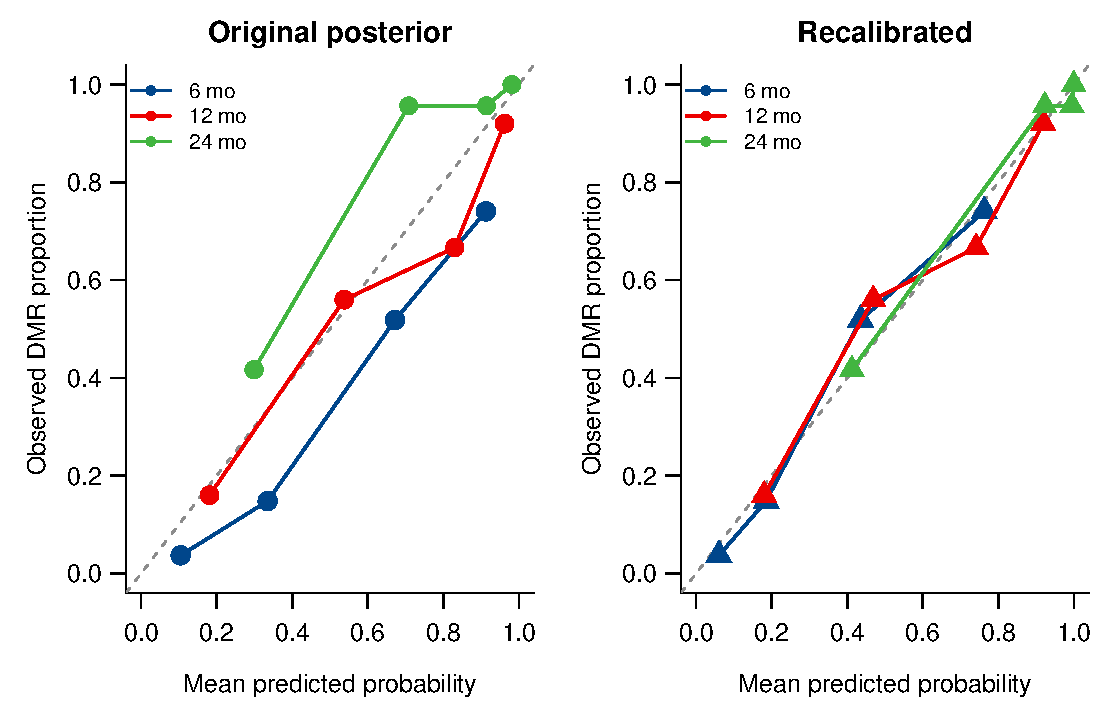
\includegraphics[width=0.96\linewidth]{figure_13_dynamic_prediction_calibration.pdf}
\caption{Development-cohort dynamic DMR calibration before and after horizon-specific logistic recalibration. Points represent quantile-based prediction bins, with point size reflecting bin size. The diagonal line indicates perfect calibration.}
\label{fig:dynamic-prediction-calibration}
\end{figure}

The dynamic prediction dataset contained 300 eligible landmark-horizon records. When pooled by horizon, the original posterior predictions overpredicted 6-month DMR probability (mean predicted 0.506 versus observed 0.361; Brier score 0.179) and modestly overpredicted 12-month DMR probability (0.626 versus 0.576; Brier score 0.162). At the 24-month horizon, the original posterior underpredicted DMR probability (0.721 versus 0.828; Brier score 0.081). Horizon-specific recalibration aligned mean predicted probabilities with observed event rates and improved apparent Brier scores, particularly for the 6-month horizon (0.157 after recalibration) and 24-month horizon (0.055 after recalibration). Bootstrap optimism-corrected recalibrated Brier scores were 0.167, 0.172, and 0.063 for the 6-, 12-, and 24-month horizons, respectively.

The recalibration coefficients reflected horizon-specific miscalibration. The estimated recalibration intercepts were \(-0.91\), \(-0.26\), and \(1.12\) for 6-, 12-, and 24-month horizons, respectively, with corresponding slopes of 0.85, 0.81, and 1.81. These results suggest that a single uncalibrated cumulative DMR probability is insufficient for patient-level dynamic use and that horizon-specific recalibration is needed before clinical interpretation.

Exploratory decision-curve analysis was generated but not emphasized because no validated clinical action threshold was prespecified for changing monitoring or treatment decisions. The dynamic predictions should therefore be interpreted as development-stage monitoring-support estimates rather than a treatment-decision rule.

\paragraph{Limitations.}
This dynamic prediction analysis is internal and exploratory. The saved posterior draws use patient-specific random effects estimated from the full longitudinal record, so the apparent performance may be optimistic relative to a prospective setting in which only MRD measurements up to landmark \(s\) are available. Recalibration was performed in the same cohort, and the bootstrap correction estimated optimism only for the recalibration layer; the full Bayesian joint model was not refitted in bootstrap or leave-one-patient-out samples. DMR onset was documented only at monitoring visits, so the evaluated outcome was documented DMR by the prediction horizon rather than exact biological onset. The later landmark strata were sparse, and no external validation cohort was available. External validation and prospective recalibration are required before using dynamic probabilities as clinical thresholds.
